\documentclass[twocolumn,10pt]{article}

\usepackage[utf8]{inputenc}
\usepackage[T1]{fontenc}
\usepackage[margin=2cm]{geometry}
\usepackage{times}
\usepackage{microtype}
\usepackage{booktabs}
\usepackage{graphicx}
\usepackage[authoryear,round,sort&compress]{natbib}
\usepackage[hidelinks]{hyperref}
\IfFileExists{xurl.sty}{\usepackage{xurl}}{}

\setlength{\columnsep}{0.22in}
\setlength{\textfloatsep}{7pt plus 1pt minus 2pt}
\setlength{\floatsep}{6pt plus 1pt minus 2pt}
\setlength{\intextsep}{6pt plus 1pt minus 2pt}
\setlength{\abovecaptionskip}{3pt}
\setlength{\belowcaptionskip}{0pt}
\makeatletter
\long\def\@makecaption#1#2{%
  \vskip\abovecaptionskip
  \small
  \sbox\@tempboxa{\textbf{#1.} #2}%
  \ifdim \wd\@tempboxa >\hsize
    \textbf{#1.} #2\par
  \else
    \global \@minipagefalse
    \hb@xt@\hsize{\hfil\box\@tempboxa\hfil}%
  \fi
  \vskip\belowcaptionskip}
\renewcommand\section{\@startsection{section}{1}{\z@}%
  {-1.2ex \@plus -0.4ex \@minus -.2ex}%
  {0.55ex \@plus .2ex}{\normalfont\large\bfseries}}
\renewcommand\subsection{\@startsection{subsection}{2}{\z@}%
  {-0.9ex \@plus -0.3ex \@minus -.2ex}%
  {0.35ex \@plus .15ex}{\normalfont\normalsize\bfseries}}
\makeatother

\title{\vspace{-1.2em}Structure or Compute?\\
A Preregistered, Budget-Matched Audit of an Agentic Workflow}
\author{C\'edric Firek\\ETH Z\"urich\thanks{Code, preregistration (tag prereg-v1), raw traces, and an interactive dashboard: \url{github.com/CedricEPFL/agent-xray}. Experiments were AI-assisted (implementation and dual-model audit pre-screening); all audit verdicts were author-confirmed.}}
\date{}

\begin{document}
\maketitle

\begin{abstract}
Agentic workflows, including critique--revision--voting pipelines and automatically searched systems, are reported to beat single LLM calls. Comparisons rarely hold inference budget constant, report paired uncertainty, or check label integrity. I ran a preregistered, budget-matched audit on MATH-500 using gemini-3.1-flash-lite. The primary contrast compared a generate--critique--revise--vote workflow against dollar-matched self-consistency on hard strata (levels 4--5, $n=248$ pairs): +0.4 percentage points (pp), 95\% CI $[-2.4,+2.8]$, exact McNemar $p=1.0$. In a calibration-matched escalation comparison with arm-specific gates, the workflow arm's point estimate was lower (78.1\% vs.\ 83.6\%, $n=73$, $p=0.29$, exploratory). Exploratory agreement-gated escalation reached within 0.4pp of the workflow at 58\% of its cost. A blind human-confirmed audit found 0 of 25 unanimous ``model failures'' genuine: 20 were scorer artifacts, 3 wrong gold labels, and 2 broken problems. Total cost was \$49.50.
\end{abstract}

\section{Introduction}
Agentic LLM research often adds structure to inference. Manual multi-agent systems coordinate specialist roles, debate, or software-engineering procedures \citep{wu2023autogen,hong2024metagpt}. Search methods optimize workflow graphs or agent architectures \citep{hu2025adas,zhang2025aflow,zhuge2024gptswarm,zhang2025maas}. These systems can improve headline accuracy, but the relevant comparison is not structure versus nothing. It is structure versus the same inference budget spent on simpler calls.

The empirical record already hints that this distinction matters. AFlow reports a +0.8pp gain over a plain call on GSM8K with gpt-4o-mini \citep{zhang2025aflow}. On the same model and benchmark, its plain-call baseline is 92.7\%, whereas MaAS reports 87.45\%, a 5.3pp gap \citep{zhang2025maas}. Such differences are larger than many reported workflow gains. They can arise from prompts, scoring, decoding, or implementation details, and they make unpaired headline comparisons weak evidence for structure.

This paper audits one concrete agentic workflow under a preregistered, budget-matched design. The motivation follows four concerns in recent evaluation work: cost-controlled agent evaluation \citep{kapoor2024agents}, failure modes in multi-agent LLM systems \citep{cemri2025mast}, nonmonotone scaling in compound inference systems \citep{chen2024more}, and the need to separate test-time compute from orchestration. The contributions are: (i) a preregistered primary contrast whose result is statistically null; (ii) an exploratory escalation experiment; (iii) a label and scorer integrity audit with an unbiased random bound; and (iv) an open instrument with harness, budget guards in the call path, analysis, and dashboard.

\section{Experimental Design}
\paragraph{Task and model.}
All experiments used gemini-3.1-flash-lite at temperature 0.7 with at most 2048 tokens per call. The benchmark was MATH-500, the 500-item subset introduced by \citet{lightman2024verify} from MATH \citep{hendrycks2021math}. All 500 items were evaluated with seed 42.

\paragraph{Systems.}
The baselines were chain-of-thought at one sample (CoT@1; \citealp{wei2022cot}) and self-consistency \citep{wang2023selfconsistency} with 3, 9, or budget-calibrated samples. SC@budget used $N=12$, fixed by a 20-item cost-only calibration that matched the workflow's realized dollar cost. The workflow drew three initial candidates; each candidate passed through generate, critique, and revise; an LLM majority vote selected the final answer. The critique and revision operator followed the same broad design principle as self-refinement \citep{madaan2023selfrefine}.

Two escalation systems probed structure at a disagreement boundary. Each arm first ran its own SC@3 and escalated only when that arm's three answers disagreed. The \textsc{esc}$\to$\textsc{workflow} arm sent flagged items into the full workflow. The \textsc{esc}$\to$\textsc{sc} arm bought 17 additional samples, calibrated to the workflow arm's mean escalation cost.

\paragraph{Instrument.}
Budget guards were evaluated in the call path (\$60 warn, \$80 stop, \$100 assert). An append-only per-call ledger recorded tokens, dollars, latency, endpoint version, and finish reason. Problem-major checkpointing preserved all-system coverage in partial runs, and every item logged its scorer method.

\paragraph{Preregistration and scoring.}
Hypotheses, analysis code, and the minimum detectable effect were registered before data collection at a public git tag, following the logic of preregistered confirmatory analysis \citep{nosek2018prereg}. The preregistration stated an MDE of approximately 6pp at discordance $q=0.10$.

Scoring used symbolic equivalence in SymPy with a normalized fallback. The per-item scoring method was logged: 93.2\% SymPy, 2.6\% string match, and 4.2\% no-method outcomes. For paired tests, items where both systems' answers could not be scored by any method were excluded and reported. Truncations were at most two calls per system, no safety blocks occurred, and failures were scored conservative-incorrect; sensitivity was unaffected. Paired contrasts used exact McNemar tests \citep{mcnemar1947} and 10{,}000 item-level paired bootstrap resamples.

\paragraph{Pilot.}
A GSM8K pilot with $n=11$ showed identical accuracy for all seven systems. The sole common miss was a wrong gold label. This motivated the audit of scorer artifacts and labels.

\begin{table}[t]
\centering
\caption{Accuracy and mean cost on all 500 MATH-500 items, repeat 0. Cost is millidollars per problem.}
\label{tab:main}
\small
\begin{tabular}{lcc}
\toprule
System & Accuracy (\%) & Cost (m\$) \\
\midrule
CoT@1 & 88.2 & 0.81 \\
SC@3 & 90.0 & 2.46 \\
\textsc{esc}$\to$\textsc{workflow} & 91.4 & 4.27 \\
\textsc{esc}$\to$\textsc{sc} & 92.0 & 5.37 \\
SC@9 & 91.2 & 7.33 \\
Workflow & 92.4 & 9.24 \\
SC@budget & 92.0 & 9.78 \\
\bottomrule
\end{tabular}
\end{table}

\section{Results}
\subsection{Primary Preregistered Contrast}
Table~\ref{tab:main} shows the all-item cost--accuracy frontier for repeat 0, and Figure~\ref{fig:pareto} visualizes the same tradeoff. The preregistered primary contrast used hard MATH levels 4--5. After excluding 14 items where both systems' answers could not be scored by any method, the paired set had $n=248$ items. The workflow scored 93.5\%; SC@budget scored 93.1\%. The difference was +0.4pp, with 95\% paired-bootstrap CI $[-2.4,+2.8]$. Discordants were 6/5, and the exact McNemar test gave $p=1.0$.

Three full repeats put the point estimate in context. Workflow accuracy was 92.4\%, 92.0\%, and 92.8\% (SD 0.4pp). SC@budget accuracy was 91.8\%, 91.8\%, and 92.0\% (SD 0.1pp). The preregistered effect estimate is therefore within run-to-run noise.

\begin{figure}[t]
\centering
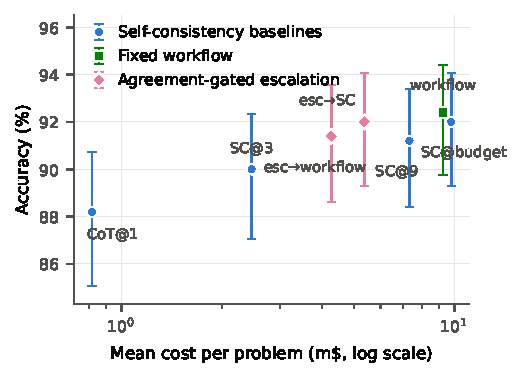
\includegraphics[width=\columnwidth]{figures/fig_pareto.pdf}
\caption{Accuracy--cost frontier on MATH-500.}
\label{fig:pareto}
\end{figure}

\subsection{Exploratory Structure Isolation}
This secondary analysis was exploratory. The all-level paired escalation comparison was also null. \textsc{esc}$\to$\textsc{workflow} scored 95.2\%, and \textsc{esc}$\to$\textsc{sc} scored 95.8\% on $n=480$ paired items. The difference was $-0.6$pp, 95\% CI $[-1.9,+0.6]$, with $p=0.51$.

The gates were arm-specific. The workflow arm escalated 66/500 items (13.2\%); the SC arm escalated 71/500 (14.2\%). Their overlap was 39 items and their union was 98 items. In levels 4--5, the union contained 77 items and $n=73$ after exclusions. On these hard-strata items flagged by either arm's own gate, the workflow arm scored 78.1\% and the SC arm scored 83.6\%. Discordants were 2/6, and $p=0.29$.

This calibration-matched, arm-specific-gate comparison is suggestive, not confirmatory. The realized mean incremental cost on escalated items was \$0.01385 for the workflow arm and \$0.02053 for the SC arm, 48\% higher despite calibration. The SC arm's higher realized spend partly confounds its higher point estimate. Still, \textsc{esc}$\to$\textsc{sc} reached 92.0\% accuracy at 58\% of the workflow's cost. Routing easy instances to cheap calls and spending more only on hard instances is not new \citep{chen2023frugalgpt,aggarwal2024automix}; here, the exploratory gate-level result motivates a shared-gate, realized-cost-matched follow-up.

\subsection{Exploratory Label and Scorer Integrity}
This secondary audit split failures into consensus flags and a random sample. Among 25 consensus flags, none was a genuine model failure. Twenty were scorer artifacts, three were wrong gold labels, and two were broken problems. Figure~\ref{fig:audit} summarizes the audit outcomes. One GSM8K gold solution computed $750+430+400+700=2280$, using a \$400 increment rather than the intended \$300 amount; the correct total is 2180, produced by every system.

\begin{figure}[t]
\centering
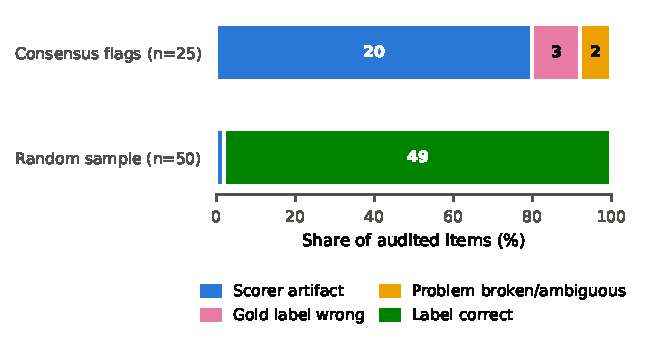
\includegraphics[width=\columnwidth]{figures/fig_audit.pdf}
\caption{Human-confirmed audit outcomes for consensus flags and random checks.}
\label{fig:audit}
\end{figure}

The random audit checked 50 items: 49 were clean and one was a scorer artifact. It found 0/50 label errors, giving a one-sided 95\% upper bound of 5.8\%. The adjudication protocol used two model families to solve all 75 audited cases independently; they agreed on 69/75. All verdicts were author-confirmed and blind to system identity.

A GSM8K anchor with $n=100$ showed the same pattern under saturation. CoT@1 reached 94\% at \$0.24m per problem. The workflow reached 93\% at \$3.58m. Removing the critique operator reached 96\%. Structured variants had lower point estimates than simpler baselines on this saturated anchor.

\subsection{Power Reality}
This design calculation is descriptive. The primary study was powered only for large effects. With $n=248$ and discordance $q=0.10$, the MDE is approximately 6pp. Table~\ref{tab:power} gives paired-item requirements for smaller effects. Effects in the 0.5--3pp range, common in workflow papers, are therefore undetectable at any affordable sample size in this setting, including in the original papers.

\begin{table}[t]
\centering
\caption{Pairs required for two-sided $\alpha=.05$, power .80.}
\label{tab:power}
\footnotesize
\setlength{\tabcolsep}{3.5pt}
\begin{tabular}{lccc}
\toprule
Effect & $q=.05$ & $q=.10$ & $q=.20$ \\
\midrule
$\delta=1$pp & 3925 & 7849 & 15698 \\
$\delta=2$pp & 981 & 1962 & 3925 \\
$\delta=3$pp & 436 & 872 & 1744 \\
$\delta=6$pp & 109 & 218 & 436 \\
\bottomrule
\end{tabular}
\end{table}

\section{Discussion and Limitations}
The main result is not that agentic structure cannot help. It is that this workflow did not beat budget-calibrated sampling on the preregistered hard-strata contrast. For this task and model, the primary contrast provides no evidence that the tested critique--revision workflow outperforms budget-calibrated sampling.

The study has narrow scope. It uses one model, one workflow family, and math-only benchmarks. Costs use list-price accounting. Prompts were frozen from the pilot for both arms. The results do not preclude structure paying off on tool-use or long-horizon tasks, where state, decomposition, and external actions may be the bottleneck.

The evaluation recommendations are direct. Workflow papers should report budget-matched baselines, paired tests with run variance, label and scorer audits, and preregistered confirmatory contrasts when the main claim is comparative \citep{kapoor2024agents,nosek2018prereg}. Disclosed deviations were: an initial mislaunch at $n=50$ stopped after 57 calls (\$0.027; corrected from an earlier mid-flight reading) and relaunched at $n=500$; S1 gates were arm-specific rather than shared, with realized escalation costs diverging 48\% from calibration, leaving the shared-gate, realized-cost-matched version as future work; and the three-run variance series was executed as a separate keyed run, whose repeat 0 differs from the primary trace by one SC@budget item (91.8\% vs.\ 92.0\%). The primary analysis uses the original preregistered trace.

\section{Conclusion}
Under a preregistered dollar match, the tested workflow did not outperform self-consistency. Exploratory escalation results were lower for the workflow arm but confounded by arm-specific gates and realized cost divergence. Small workflow gains require paired, audited, budget-controlled evidence before they should be attributed to structure.

\clearpage
\bibliographystyle{abbrvnat}
\bibliography{refs}

\end{document}
